\chapter{Cahier des charges}
% Partie dans laquelle on explique les features / requirements attendues
% On y trouve sans doute :

\epigraph{<< Les choses paraissent simples jusqu'à ce qu'on commence à les analyser >>}{Audrey Niffenegger}

\section{Analyse fonctionnelle}

\subsection*{Séparation des tâches}

Comme expliqué par les Echos\cite{SOD}, il s'agit  "d'un concept qui requière différents acteurs possédant des rôles et responsabilités différents pour la réalisation d’un ensemble de tâches dont l’exécution par un unique acteur pourrait potentiellement conduire à des fraudes ou des erreurs". \\


En effet, ce catalogue participatif nécessite un certain nombre de garde-fous afin de maintenir un outil qui dispose de ressources aussi bien de manière qualitative que quantitative. Notre analyse nous a permis d'isoler ces 4 types d'utilisateurs qui disposent de privilèges de manière incrémentale (en plus de disposer de leurs privilèges propres, chacun hérite aussi de ceux du précédent de la présente liste) :


\begin{itemize}
    \item Visiteur : Il s'agit d'un utilisateur non inscrit à notre plate-forme. Il ne peut rechercher et consulter que les fiches de ressources validés par un administrateur.
    \item Utilisateur : Il s'agit d'un utilisateur  inscrit à notre plate-forme. Celui-ci peut proposer des nouvelles ressources ainsi que de maintenir les fiches dont il est le créateur.
    \item Administrateur : Celui-ci crée/modifie des ressources de toute nature (fiches proposées par les utilisateurs, mots clés et catégories de mots clé), en plus de classifier les fiches.
    \item Super Administrateur : Celui-ci dispose du droit de supprimer de manière définitif les différentes ressources de notre plate-forme.
\end{itemize}

\pagebreak

\subsection*{État d'une fiche}

Durant notre analyse, nous avons été confrontés à de nombreuses questions autour du processus 





C'est pourquoi nous avons . Nous utiliserons un diagramme UML à états pour représenter les états et les principales transitions :

% width=\textwidth,height=\textheight,keepaspectratio
\begin{figure}[H]
    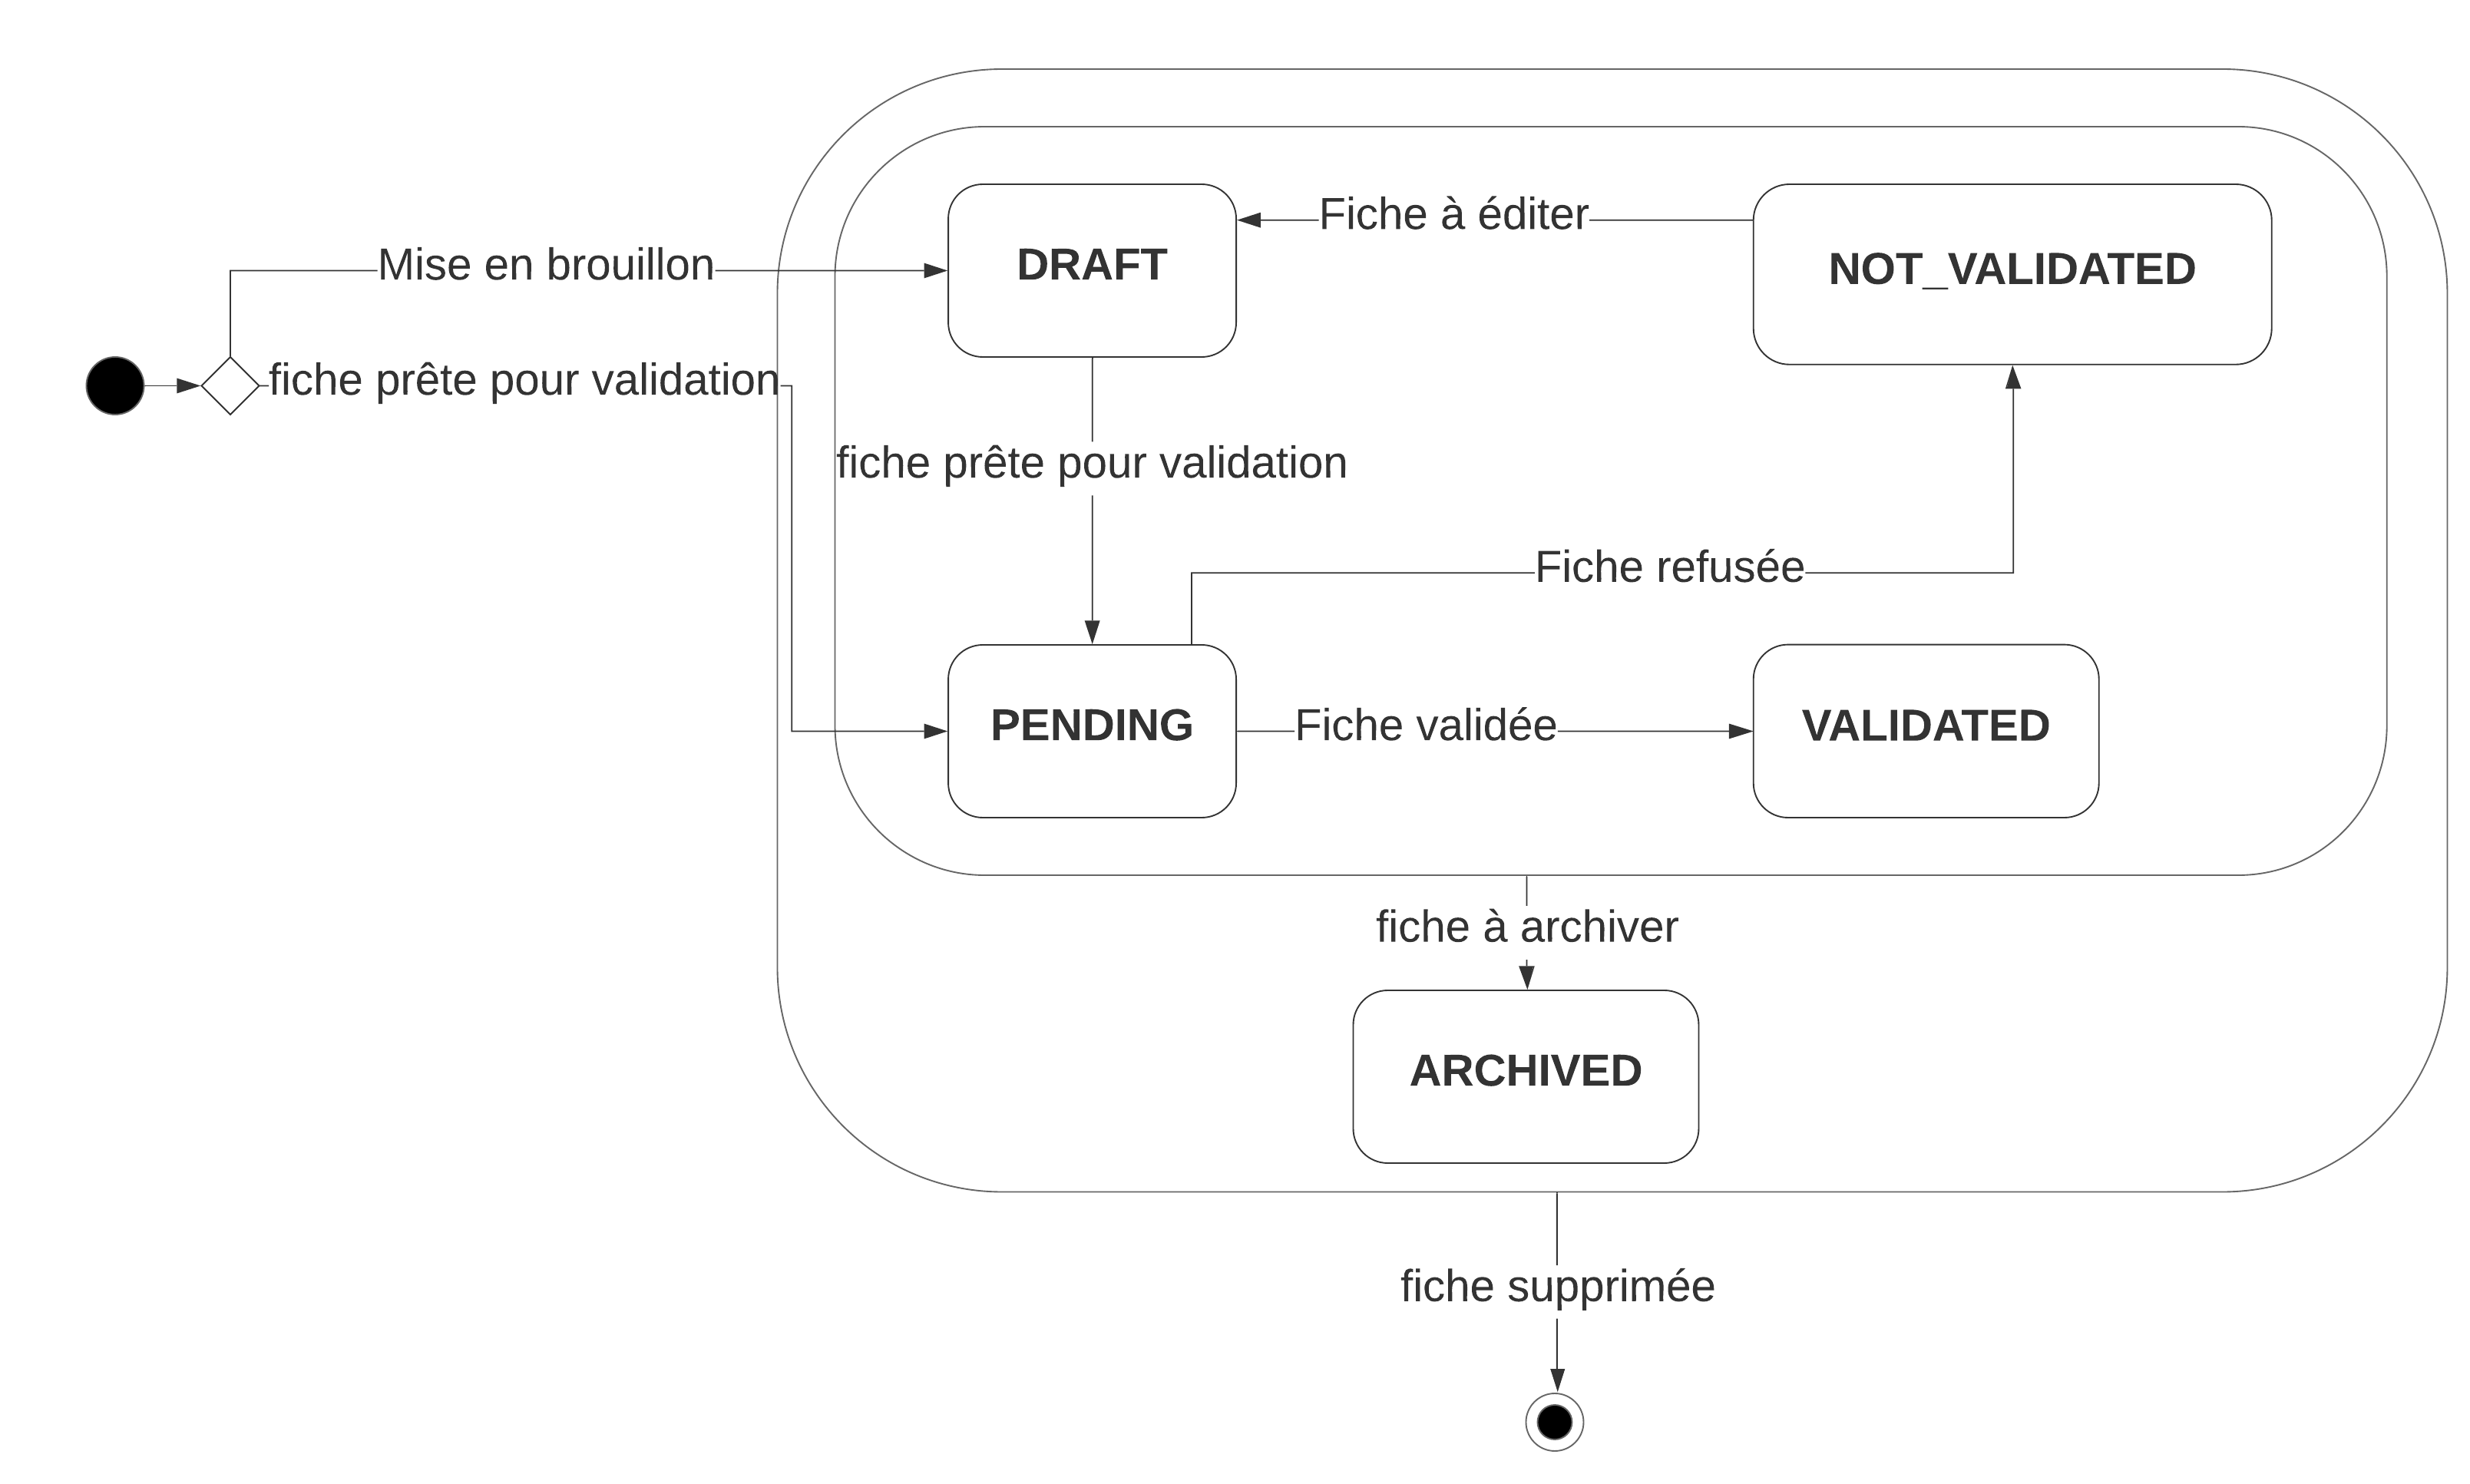
\includegraphics[width=\textwidth,height=\textheight,keepaspectratio]{images/StateFiches.png}
    \caption{Diagramme UML à états pour l'état d'une fiche}
    \label{pic:stateDiagramForFiches}
\end{figure}


% Image

\subsection*{Status des mots clés}



\subsection*{Fonctionnalités}

TODO


% Image

% Users
% Exercise states
% Tag states
% Fonctionnalités 

% - diagrammes de cas d'utilisations ( + visuel qu'une liste de user stories )
% - explications des différents rôles dans l'application ( guest, user, admin )

\section{Analyse non-fonctionnelle}
% On explique ici ( design, ergonomie )
% Donner les critères d'ergonomie
% Pas forcément des tonnes de page : à priori 3-4 max devraient suffire

\section {Contraintes}
% Expliquer les contraintes :
%    - Maintenabilité / Extensibilité  du code
%    - Gestion simple du système ( quand Mens disait que les admins ne devaient pas avoir à toucher à la DB pour faire x ou y truc )
%    - Interface orienté vers l'UX ( une jolie instruction UI VS UX
%    - etc...